% !TeX encoding = utf8
% !TeX spellcheck = en_US

\section{Methods}

\subsection{Participants}
Two male participants 25 years of age were recruited by the ARTORG Center for Biomedical Engineering Research. These two participants were healthy and did not suffer from any known pre-existing medical conditions. This study was conducted at the NeuroTec research facility in the Swiss Institute for Translational and Entrepreneurial Medicine (sitem-insel) and at the Stadion Neufeld, both located in Bern, Switzerland.

\subsection{Data collection}
The AX6 Axivity 6-axis logging movement sensor (Newcastle, United Kingdom) was used to collect accelerometer data in this study. The puck has dimensions of 23 $\times$ 32.5 $\times$  8.9\,mm and a weight of 11\,g.

On both the left and right legs, the sensors were placed on the anterior aspect of the tibia, 7\,cm above the lateral malleolus as depicted in Figure \ref{fig:sensorplacement}. To affix the sensors, a one-sided adhesive interface was utilized and the sensor was placed beneath this adhesive. 

Positioning was selected so that the walking direction would follow the z-direction, as depicted in Figure \ref{fig:sensorplacement}, and based on findings from a prior systematic review indicating that IMU placement closer to the ground enhances gait event detection \cite{pacini_panebianco_analysis_2018}.

\begin{figure}[h]
	\centering
	\includegraphics[width=0.6\linewidth]{"Figures/SensorPlacement"}
	\caption{Sensor Placement \cite{noauthor_foot_nodate}}
	\label{fig:sensorplacement}
\end{figure}

After sensor placement, the participants were asked to walk, at what they consider their regular walking speed, one lap around a 400\,m track. Before starting and at the end of the walk, the participants were asked to jump in place three times. The idea was to set reference points to facilitate later analysis since this would create evident signals in the accelerometer data.

The step counter IOS app Counter+ developed by Yan Kin LEUNG was used to establish a ground truth of the actual number of steps walked during the experiment. The participants were asked to use this application to count their steps while walking. Additionally, the participants were followed by a researcher also counting their steps using the same application. Importantly, the follower carefully remained behind the participant and out of sight in order to reduce any chance of influencing the participant's gait. The mean from both counts was taken and is displayed in Table \ref{tab:results} in the row named \emph{counted total steps}.

\subsection{Parkinson's disease patient data}
In collaboration with the Gerontechnology and Rehabilitation Research Group of the ARTORG Center for Biomedical Engineering Research and the Division of Cognitive and Restorative Neurology within the medical faculty at the University of Bern, we were kindly provided with previously collected accelerometer data from a patient suffering from Parkinson's disease. 

The Parkinson's disease patient's data was recorded over a five minute time period during which the patient walked back and forth in a 30\,m long hallway. Due to these changes in direction, the signal was very inconsistent and discontinuously periodic. Therefore, to facilitate the analysis, only a 24 second interval from the signal was selected.


\subsection{Data processing}
The accelerometers were setup and configured using the AX3/AX6 OMGUI Configuration and Analysis Tool which is an open source application developed by the Open Movement Team at Newcastle University, United Kingdom. This application allowed the data to be exported as CSV files which was later processed with Python v3.12. Additional packages, as displayed in Table \ref{tab:packages}, were used to further process the data.

\begin{table}[H] % Full width table (notice the starred environment)
	\caption{Additional packages for data processing.}
	\centering % Horizontally center the table
	\begin{tabularx}{\linewidth}{X|X|} % Manually specify column alignments with L{}, R{} or C{} and widths as a fixed amount, usually as a proportion of \linewidth
		\toprule
		Package & Version \\
		\midrule
		Matplotlib & 3.8.0 \\
		NumPy & 1.26\\
		Pandas & 2.2.1\\
		SciPy & 1.12.0\\
		Sensor Motion & 1.1.4\\
		\bottomrule
	\end{tabularx}
	\label{tab:packages}
\end{table} 

\subsection{Filtering}
In order to reduce the noise, the accelerometer data was filtered with a third-order low-pass Butterworth filter with a 5\,Hz cutoff frequency. In order to remove the DC component of the signal, a third-order high-pass Butterworth filter with a 0.5\,Hz cutoff frequency was applied. Together, these filters band-passed the signal. These cutoff values were chosen so that the three greatest amplitude frequencies were contained in the smoothed signal. This was done by taking the Fast Fourier Transform (FFT) of the signal to go from the time domain to the frequency domain. 

For visualization purposes, sample FFT plots, before and after filtering, can be seen in Figure \ref{fig:fft_plot}. The sampling rate of the accelerometers was kept at the default value of 100\,Hz, which is adequate for studies of human movement. Note the 50\,Hz frequency axis due to the Nyquist-Shannon sampling theorem which states that the sampling rate must be two times the largest frequency \cite{mcclellan_dsp_2017}.

\begin{figure}[H]
	\centering
	\begin{subfigure}{\linewidth}
		\centering
		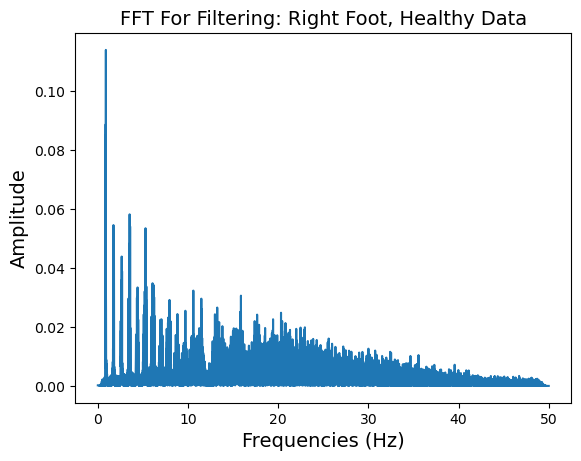
\includegraphics[width=\linewidth]{Figures/fft_plot.png}
		\caption{FFT plot before filtering.}
		\label{fig:fft_plot_before}
	\end{subfigure}\vfill
	\begin{subfigure}{\linewidth}
		\centering
		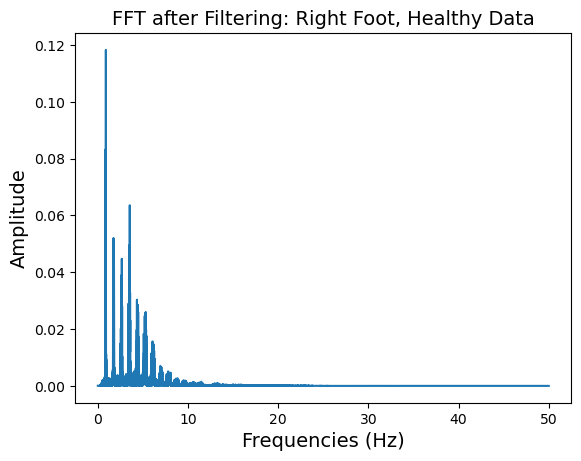
\includegraphics[width=\linewidth]{Figures/fft_after_filter_plot.png}
		\caption{FFT plot after filtering.}
		\label{fig:fft_plot_after}
	\end{subfigure}
	\caption{FFT plots of the signal from participant B.}
	\label{fig:fft_plot}
\end{figure}

\subsection{Peak detection}
The definitions for initial contact (IC) and terminal contact (TC) provided by Gottlied and colleagues were used. Initial contact is defined as the moment in the gait cycle when the foot first makes contact with the ground, corresponding to heel-strike during forward walking (FW). Terminal contact is defined as the instant in the gait cycle when the foot completely lifts off the ground, corresponding to toe-off during FW \cite{gottlieb_agreement_2020}.
\begin{figure}[h]
	\centering
	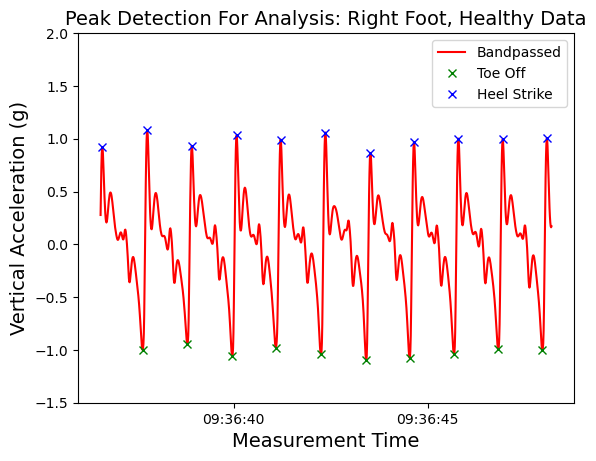
\includegraphics[width=\linewidth]{Figures/peak_detection.png}
	\caption{Peak and valley detection for participant B.}
	\label{fig:peak_detection}
\end{figure}
The \emph{find\_peaks} method, available in the Sensor Motion Python package, was used to detect peaks in the accelerometer signal data. This method employs advanced algorithms to identify significant changes or peaks within the signal, crucial for recognizing distinct motion patterns or events. By specifying parameters such as minimum peak height or distance between peaks (number of samples), the peak detection process was tailored to suit the specific analysis requirements. The values selected for these parameters can be found in Table \ref{tab:peak_values}.
\begin{table}[H] % Full width table (notice the starred environment)
	\caption{Values for peak and valley detection.}
	\centering % Horizontally center the table
	\begin{tabularx}{\linewidth}{l|c|c|c|} % Manually specify column alignments with L{}, R{} or C{} and widths as a fixed amount, usually as a proportion of \linewidth
		\toprule
		& Parkinson's  & Part. A & Part. B \\
		\cmidrule(r){2-4}
		Distance & 75 & 50 & 50\\
		Peak height& 0.50 & 0.75 & 0.65\\
		Valley height & 0.50 & 0.68 & 0.70\\
		\bottomrule
	\end{tabularx}
	\label{tab:peak_values}
\end{table} 

Additionally, visual inspection, as shown in Figure \ref{fig:peak_detection}, was necessary to confirm the success of the method. This approach facilitated the extraction of key features from the accelerometer data, enabling the characterization and interpretation of various motion-related phenomena with precision and accuracy. 

\subsection{Calculation of temporal gait parameters}
Once the peaks were obtained, calculating steps is quite straightforward since it entails just counting the number of peaks found.

Zanardi and colleagues describe certain temporal gait parameters in which a meta-analysis showed a difference between Parkinson's disease patients and healthy controls \cite{zanardi_gait_2021}. Therefore, given what was attainable from the obtained data, some of these parameters, such as mean swing time, stance time, stride time and cadence were calculated. The calculations for these parameters can be found in Table \ref{tab:calculaitons} \cite{grucci_gait_2019}.

 \begin{table}[H] % Full width table (notice the starred environment)
 	\caption{Calculations for the temporal parameters which include IC and TC of the foot that is leading (IC1 and TC1) and the foot that is lagging (IC2 and TC2).}
 	\centering % Horizontally center the table
 	\begin{tabularx}{\linewidth}{X|c|c|} % Manually specify column alignments with L{}, R{} or C{} and widths as a fixed amount, usually as a proportion of \linewidth
 		\toprule
 		Temporal parameters & Leading & Lagging \\
 		\midrule
 		Swing time (s) & IC1 - TC1 & IC2 - TC2\\
 		Stance time (s)  & TC1 - IC1 & TC2 - IC2\\
 		Stride time (s)  & IC1 - IC1 & IC2 - IC2\\
 		Cadence (steps/min) & \multicolumn{2}{c|}{2*60/(mean stride time)}\\
 		\bottomrule
 	\end{tabularx}
 	\label{tab:calculaitons}
 \end{table} 

Swing time is defined as the duration of when the reference limb is not in contact with the ground whereas, conversely, during stance time, the reference limb is in contact with the ground. Stride time is defined as the duration between the initial contact of a foot and the ensuing initial contact of the ipsilateral foot. Cadence, as the units may suggest, is the number of steps taken during an interval of time, which is per minute in this case \cite{webster_principles_2019}.


%Not going into report but leaving for information
%Some important gait parameters are speed, stride length, cadence, step width, single and double support time, swing time, range of motion for the hip, knee and ankle and the angle at initial contact for the hip, knee and ankle \cite{zanardi_gait_2021}.

\subsection{Removal of Outliers}
In full transparency, during the analysis of the gait data, outliers were observed and subsequently removed - for swing time, 3 outliers for participant A and 2 outliers for participant B, and for stance time, 2 outliers for both participants.

Outliers can heavily influence summary statistics such as mean, standard deviation, and correlation coefficients. By removing outliers, more accurate estimates of these statistics can be obtained, which in turn lead to more reliable interpretations of the data. As such the samples which were three standard deviations larger or smaller than the mean were removed \cite{osborne_power_nodate}.

\subsection{Accuracy of Step Counter}
In order to get some sort of a metric to describe the validity of accelerometers as a step counter, the error rate was calculated using the Equation \eqref{eqn:accuracyEquation} described by Cleland and colleagues \cite{cleland_effects_2012}.
\begin{equation}
	\label{eqn:accuracyEquation}
	Accuracy = \biggl(1 - \frac{C_s - A_s}{A_s}\biggr) \times 100
\end{equation}
where $C_s$ is the calculated steps from the accelerometer data and $A_s$ is the steps counted, which is taken here as the ground truth. 
















